\documentclass[11pt,fleqn,dvipsnames,usenames]{article}

% to keep this file less overwhelming
% packages to include

\usepackage[dvipsnames, table]{xcolor}

\usepackage{
  amsmath,
  amssymb, 
  arydshln, % for hyphenated lines in block matrices
  fancyhdr, % needed for header at top of each page
  graphicx, % to include pictures
  hyperref, % for hyper links
  mathtools, % for a longer arrow
  multicol, % displaying enumerates and itemizes into multiple columns
  multirow, % for tables
  multido, % for TOC
  pgfplots, % for axis environment within tikz pictures
  systeme,
  tikz,
}

\usepackage[inline, shortlabels]{enumitem}


% global constants
\newcommand{\term}{Fall 2024}
\newcommand{\course}{Math 2210}

% mathbb aliases
\newcommand{\COMPLEX}{\mathbb{C}}
\newcommand{\C}{\COMPLEX}
\newcommand{\REAL}{\mathbb{R}}
\newcommand{\R}{\REAL}
\newcommand{\RATIONAL}{\mathbb{Q}}
\newcommand{\Q}{\RATIONAL}
\newcommand{\INTEGER}{\mathbb{Z}}
\newcommand{\Z}{\INTEGER}
\newcommand{\ZN}{\INTEGER_{n}}
\newcommand{\NATURAL}{\mathbb{N}}
\newcommand{\N}{\NATURAL}

\newcommand{\ZX}{\Z[x]}
\newcommand{\ZNX}{\ZN[x]}
\newcommand{\QX}{\Q[x]}
\newcommand{\RX}{\R[x]}
\newcommand{\CX}{\C[x]}
\newcommand{\CZ}{\C[z]}

% complex number aliases
\newcommand{\RE}[1]{\text{Re}\left(#1\right)}
\newcommand{\IM}[1]{\text{Im}\left(#1\right)}
\newcommand{\CC}[1]{\overline{#1}}
\newcommand{\ARG}[1]{\text{arg}\left(#1\right)}
\newcommand{\PARG}[1]{\text{Arg}\left(#1\right)}

% for financial stuff
\newcommand{\dollar}{\mathrm{\$}}

% nicer looking trig functions
\newcommand{\SIN}[1]{\sin\left(#1\right)}
\newcommand{\COS}[1]{\cos\left(#1\right)}
\newcommand{\TAN}[1]{\tan\left(#1\right)}
\newcommand{\CSC}[1]{\csc\left(#1\right)}
\newcommand{\SEC}[1]{\sec\left(#1\right)}
\newcommand{\COT}[1]{\cot\left(#1\right)}

% number theory
\newcommand{\ndiv}{|\kern-0.9ex{/}}

% automatically resize set brackets
\newcommand{\SET}[1]{\left\{#1\right\}}

% sums and products
\newcommand{\SUM}{\displaystyle\sum\limits}
\newcommand{\PROD}{\displaystyle\prod\limits}
\newcommand{\LIMIT}{\displaystyle\lim\limits}
\newcommand{\of}{\circ}
\newcommand{\restrict}[1]{\raisebox{-.5ex}{$|$}_{#1}}

% set intersection and union
\newcommand{\CAP}{\displaystyle\bigcap\limits}
\newcommand{\CUP}{\displaystyle\bigcup\limits}

% polynomials
\newcommand{\DEG}[1]{\ensuremath{\text{deg}\left(#1\right)}}

% max and min
\newcommand{\MAX}[1]{\ensuremath{\max\left\{#1\right\}}}
\newcommand{\MIN}[1]{\ensuremath{\min\left\{#1\right\}}}

% gcd and lcm
\newcommand{\GCD}[1]{\ensuremath{\text{gcd}\left(#1\right)}}
\newcommand{\LCM}[1]{\ensuremath{\text{lcm}\left(#1\right)}}

% for writing logic within mathematics environment
\newcommand{\FORALL}{\ensuremath{\text{ for all }}}
\newcommand{\FORSOME}{\ensuremath{\text{ for some }}}

% matrix notation
\newcommand{\MATRIX}[2]{\ensuremath{\left[\begin{array}{#1}#2\end{array}\right]}}
\newcommand{\COLUMN}[1]{\ensuremath{\left[\begin{array}{r}#1\end{array}\right]}}
\newcommand{\BY}{\times}

% vector notation
%\newcommand{\vv}{\overset{\rightharpoonup}}
\newcommand{\vv}[1]{{\bf #1}}
\newcommand{\arr}{\overrightarrow}

% dot product
\newcommand{\dotp}{{\scriptstyle\bullet}}

% Text macros
\newcommand{\KER}[1]{\ensuremath{\text{ker}\left(#1\right)}}
\newcommand{\IMG}[1]{\ensuremath{\text{im}\left(#1\right)}}
\newcommand{\CHAR}[1]{\ensuremath{\text{char}\left(#1\right)}}
\newcommand{\BIGO}[1]{\ensuremath{\mathcal{O}\left(#1\right)}}
\newcommand{\TR}[1]{\ensuremath{\text{tr}\left(#1\right)}}

% abbreviations
\newcommand{\ds}{\displaystyle}
\newcommand{\md}{\mdseries}

% abbreviations for vertical/horizontal spaces
\newcommand{\vsp}{\vspace{0.5cm}}
\newcommand{\smsp}{\vspace{0.25cm}} % small space
\newcommand{\vsmsp}{\vspace{0.1cm}} % very small space
\newcommand{\hsp}{\hspace{0.25cm}}

% new operators
\DeclareMathOperator\SPAN{Span}
\newcommand{\SPANOF}[1]{\ensuremath{\SPAN\left\{#1\right\}}}
\DeclareMathOperator\PROJ{proj}
\DeclareMathOperator\PERP{perp}

% underlining definitions
\newcommand{\DEF}[1]{\textbf{\ul{#1}}}

% environments
\newtheorem{theorem}{Theorem}[subsection]
\newtheorem*{theorem*}{Theorem}
\newtheorem{corollary}[theorem]{Corollary}
\newtheorem*{corollary*}{Corollary}
\newtheorem{lemma}[theorem]{Lemma}

\theoremstyle{definition}
\newtheorem{definition}[theorem]{Definition}
\newtheorem*{definition*}{Definition}
\newtheorem{example}[theorem]{Example}
\newtheorem*{example*}{Example}
\newtheorem{examples}[theorem]{Examples}
\newtheorem*{examples*}{Examples}
\newtheorem{exercise}[theorem]{Exercise}
\newtheorem*{exercise*}{Exercise}
\newtheorem{exercises}[theorem]{Exercises}
\newtheorem{remark}[theorem]{Remark}
\newtheorem{remarks}[theorem]{Remarks}

% make proof boxes solid
\renewcommand{\qedsymbol}{$\blacksquare$}

% quick abbreviations to avoid using latex environments (gradually phasing these out)
\newcommand{\analogy}{\noindent \textbf{Analogy:} }
\newcommand{\answer}{\noindent \textbf{Answer:} }
\newcommand{\answers}{\noindent \textbf{Answers:} }
\newcommand{\application}{\noindent \textbf{Application:} }
\newcommand{\background}{\noindent \textbf{Background:} }
\newcommand{\caution}{\noindent \textbf{Caution:} }
\newcommand{\conclusion}{\noindent \textbf{Conclusion:} }
\newcommand{\consequence}{\noindent \textbf{Consequence:} }
\newcommand{\convention}{\noindent \textbf{Convention:} }
\newcommand{\conventions}{\noindent \textbf{Conventions:} }
\newcommand{\crlry}{\noindent \textbf{Corollary:} }
\newcommand{\defn}{\noindent \textbf{Definition:} }
\newcommand{\details}{\noindent \textbf{Details:} }
\newcommand{\nexamples}[1]{\noindent \textbf{Examples (#1):}} 
\newcommand{\exception}{\noindent \textbf{Exception:} }
\newcommand{\nexercise}[1]{\noindent \textbf{Exercise (#1):}} 
\newcommand{\nexercises}[1]{\noindent \textbf{Exercises (#1):}} 
\newcommand{\fact}{\noindent \textbf{Fact:} }
\newcommand{\facts}{\noindent \textbf{Facts:} }
\newcommand{\fix}{\noindent \textbf{Fix:} }
\newcommand{\formula}{\noindent \textbf{Formula:} }
\newcommand{\goal}{\noindent \textbf{Goal:} }
\newcommand{\goals}{\noindent \textbf{Goals:} }
\newcommand{\hint}{\noindent \textbf{Hint:} }
\newcommand{\idea}{\noindent \textbf{Idea:} }
\newcommand{\illustration}{\noindent \textbf{Illustration:} }
\newcommand{\important}{\noindent \textbf{Important:} }
\newcommand{\lema}{\noindent \textbf{Lemma:} }
\newcommand{\midea}{\noindent \textbf{Main Idea:} }
\newcommand{\motivation}{\noindent \textbf{Motivation:} }
\newcommand{\nthm}[1]{\noindent \textbf{Theorem} (\textit{#1}):}
\newcommand{\notation}{\noindent \textbf{Notation:} }
\newcommand{\note}{\noindent \textbf{Note:} }
\newcommand{\notes}{\noindent \textbf{Notes:} }
\newcommand{\observation}{\noindent \textbf{Observation:} }
\newcommand{\observations}{\noindent \textbf{Observations:} }
\newcommand{\pict}{\noindent \textbf{Picture:} }
\newcommand{\plan}{\noindent \textbf{Plan:} }
\newcommand{\prf}{\noindent \textbf{Proof:} }
\newcommand{\problem}{\noindent \textbf{Problem:} }
\newcommand{\properties}{\noindent \textbf{Properties:} }
\newcommand{\question}{\noindent \textbf{Question:} }
\newcommand{\questions}{\noindent \textbf{Questions:} }
\newcommand{\recall}{\noindent \textbf{Recall:} }
\newcommand{\reason}{\noindent \textbf{Reason:} }
\newcommand{\reminder}{\noindent \textbf{Reminder:} }
\newcommand{\solution}{\noindent \textbf{Solution:} }
\newcommand{\nsolution}[1]{\noindent \textbf{Solution #1:} }
\newcommand{\setting}{\noindent \textbf{Setting:} }
\newcommand{\strategy}{\noindent \textbf{Strategy:} }
\newcommand{\summary}{\noindent \textbf{Summary:} }
\newcommand{\terminology}{\noindent \textbf{Terminology:} }
\newcommand{\thm}{\noindent \textbf{Theorem:} }
\newcommand{\work}{\noindent \textbf{Work:} }

% gray line across pagewidth
\newcommand{\GRAYLINE}{
  {\color{gray}\leaders\vrule width \textwidth\vskip0.4pt} % or other desired thickness
  \vskip\medskipamount % ditto
  \nointerlineskip
  \smsp
}

\usepackage[version=4]{mhchem}

% Where to look for pngs and jpegs
\graphicspath{{Images//}}

\usepackage[includehead, includefoot, left= 2cm, top =1.5cm, bottom = 1.5cm, textwidth=17.5cm]{geometry}

\usepackage{pifont, amsmath}


\pagestyle{fancy}
\fancyhf{}
\renewcommand{\headrulewidth}{1pt}
%\fancyhead[R]{\bfseries\sffamily\thepage}
%\fancyfoot[C]{\bfseries\sffamily\thepage}
\fancyhead[L]{\nouppercase{\bfseries\sffamily\leftmark}}

% used when adding fill-in-the-blanks for students
\newcommand{\blank}[1]{\underline{\hspace{#1}}}

% indents annoy me, and so does repeatedly typing \noindent
\newcommand{\p}{\noindent}

\begin{document}

\fancyhead[L]{\course}
\fancyhead[C]{
\includegraphics[width=5cm, trim= 0 0.4cm 0 0]{TRU_logo}}
\fancyhead[R]{\term}
\renewcommand{\headrulewidth}{0.4pt}

\setulcolor{red}

\setcounter{section}{1}
\section{Complex Numbers}
\setcounter{subsection}{3}
\subsection{Arguments}

\p Remember that the argument of a complex number is not unique!  For example, both $\pi/4$ and $9\pi/4$ are arguments for $1 + i$.  More generally, if $\theta$ is an argument for $z\in\COMPLEX$, then so is $\theta + 2\pi k$ for any $k\in \INTEGER$.
\vsp

\notation For any $z\in\COMPLEX$ with argument $\theta$, we may capture all of its arguments with the notation
\vspace{2cm}

\p where it is understood that $k$ varies over the set of integers.
\vsp

\fact For any $\theta\in\REAL$, there exists a unique $k^{\star}\in\INTEGER$ such that $\theta + 2\pi k^{\star}\in (-\pi, \pi]$.  In this case $\theta + 2\pi k^{\star}$ is\\
\vsmsp

\p called the \DEF{principle argument} of $z$, and is denoted by \blank{1cm}.
\vsp

\begin{examples}~
\begin{enumerate}[(a)]
\item $z = 1 + i$
\vspace{1cm}

\item $z = e^{i(5\pi/3)}$
\vspace{1cm}

\end{enumerate}
\end{examples}

\subsection{Roots of Complex Numbers}\label{rootsofunitysection}

\p For the duration of this section, $n$ shall always denote a positive integer.
%
\begin{definition*}
A complex number $z$ is said to be an $n$th root of unity if $z^{n} = 1$.
\end{definition*}
%
\begin{example*}
What are the fourth roots of unity?
\end{example*}
%
\begin{solution}
\end{solution}
\newpage

\note The fourth roots of unity are all powers of $i = e^{i(\pi/2)}$, which wrap around the unit circle in the counter-clockwise direction.
\vsp

\observations For $n\in\Z^{+}$, let $\omega = e^{i(2\pi/n)}$.
\begin{enumerate}[(1)]
\item $\omega$ is an $n$th root of unity.
\vspace{2cm}

\item $\omega^{k}$ is also an $n$th root of unity.
\vspace{2cm}

\item The only $n$th roots of unity are the complex numbers of the form $\omega^{k}$ for some $k\in\INTEGER$.
\vspace{5cm}

\item For all $k\in\Z$,
\vsp
\end{enumerate}

\begin{theorem*}\label{rootsofunityclassification}
The $n$ distinct $n$th roots of unity are given by $\omega^{k} = e^{2\pi i k/n}$, with $k\in\INTEGER$ with $0\leq k < n$, where
\begin{center}
$\omega = e^{2\pi i/n}$.
\end{center}
\end{theorem*}
\vsp

\begin{example*}\label{fifthrootsunityexample}
Find all of the fifth roots of unity.
\end{example*}
%
\begin{solution}
\end{solution}
\newpage

\p The fifth roots of unity $\omega^{0}, \omega^{1}, \omega^{2},\omega^{3}$ and $\omega^{4}$ from the previous example are sketched below on the left.  Note that they form the vertices of a regular hexagon with center of mass located at the origin, which is shown on the right.

\begin{center}
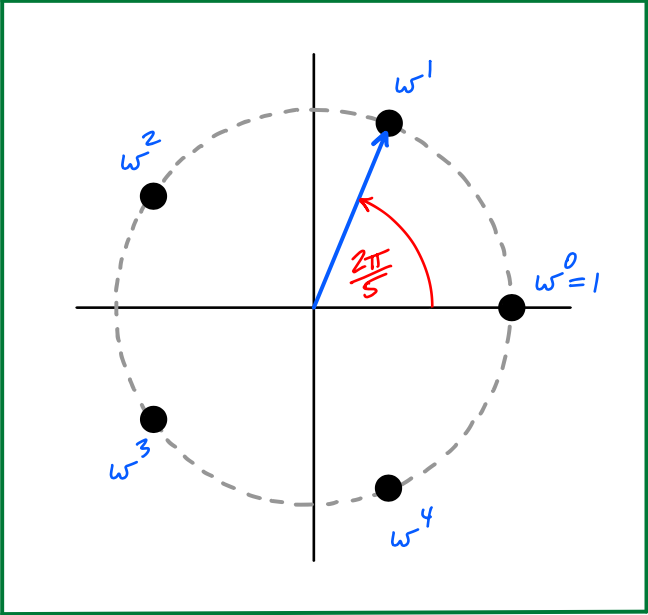
\includegraphics[width=0.3\linewidth]{fifthrootsunity}\hspace{4cm} 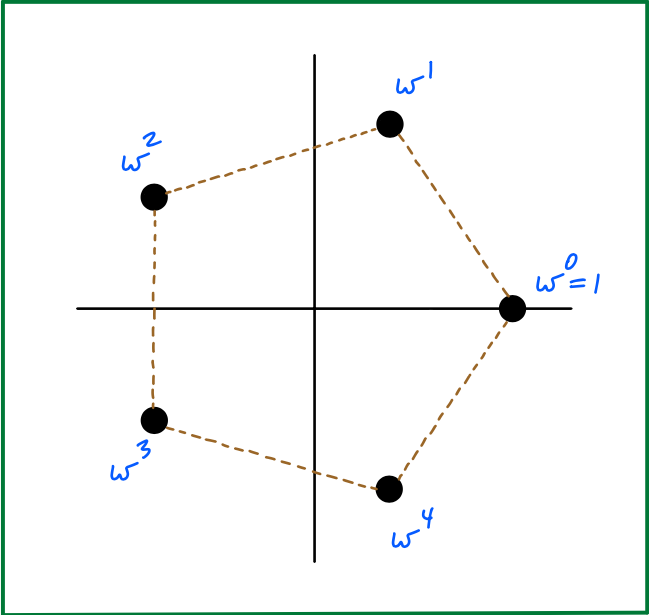
\includegraphics[width=0.3\linewidth]{fifthrootsunityhexagon}
\end{center}
%
\begin{definition*} Let $n> 1$.  A complex number $\omega\in\COMPLEX$ is a \DEF{primitive $n$th root of unity} if $\omega^{n} = 1$ and $\omega^{k}\neq 1$ whenever $0 < k < n$.
\end{definition*}
%
\begin{examples*}~
\end{examples*}
\newpage

\begin{lemma*}
Let $k\in\Z$ and $\omega = e^{i(2\pi/n)}$.  $\omega^{k} = 1$ if and only if $n|k$.
\end{lemma*}
%
\prf
\vspace{6cm}
%

\begin{theorem*}
If $\omega = e^{i(2\pi/n)}$ and $k\geq 1$ is an integer, then
\begin{center}
$\omega^{k} = e^{i(2\pi k/n)}$
\end{center}
is a primitive $n$th root of unity if and only if $\GCD{n,k} = 1$.
\end{theorem*}
\vsp

%
\begin{definition*}
Let $z = re^{i\theta}\in \C$ and $n\geq 1$ be an integer. The \DEF{complex $n$th roots} of $z$ are given by
\begin{center}
$z^{1/n} := \sqrt[n]{r}e^{i(\theta + 2\pi k)/n}$, where $k\in\SET{0, 1, \ldots, n -1}$.
\end{center}
\end{definition*}
%
\begin{example*}
Find all of the cube roots of $\sqrt{2} + i\sqrt{2}$.
\end{example*}
%
\begin{solution}
\end{solution}
\newpage

%
\begin{remark}
When seeking the $n$th roots of a complex number $z$, an alternative approach is as follows.  Find \emph{any} $n$th root of $z$ and multiply it by each of the $n$th roots of unity.
\end{remark}
%
\begin{example*}
Find all the fifth roots of $2$.
\end{example*}
%
\begin{solution}
\end{solution}



\end{document}





